\documentclass[aspectratio=169,xcolor=dvipsnames]{beamer}
\usetheme{SimplePlus}

\usepackage{hyperref}
\usepackage{graphicx} % Allows including images
\usepackage{booktabs} % Allows the use of \toprule, \midrule and \bottomrule in tables
\usepackage[brazil]{babel}

\title{Heurística de Roteamento e Alocação de \\ Fibras em Redes Ópticas}
% \subtitle{Subtitle}
\author{Diego M. A. Lütke}
\institute
{
    Escola Politécnica \\
    Pontifícia Universidade Católica do Paraná
}

\date{18 de Outubro de 2025}

\begin{document}

\begin{frame}
    % Print the title page as the first slide
    \titlepage
\end{frame}

\begin{frame}{Resumo}
    \tableofcontents
\end{frame}

\section{Introdução}\label{sec:introducao}
\begin{frame}{\ref{sec:introducao} - Introdução | Motivação e Objetivo}
  \begin{itemize}
    \item O papel crítico das redes de fibra ótpica em infraestruturas de telecom.
    \item A necessidade de eficiência e qualidade na entrega de projetos.
    \item Os impactos de uma rede desorganizada (e.g. demora em manutenções preventivas e emergenciais).
    \item Alternativas menos custosas.
  \end{itemize}
\end{frame}

\begin{frame}{\ref{sec:introducao} - Introdução | Objetivo}
  \begin{itemize}
    \item Propor uma heurística prática para roteamento físico (i.e. escolha da rota + escolha da fibra).
    \item Otimizar a escolha de rotas e a alocação de fibras disponíveis, considerando aspectos práticos da rede.
  \end{itemize}
\end{frame}

\section{Contexto e Diagnóstico}\label{sec:contexto}
\begin{frame}{\ref{sec:contexto} - Contexto e Diagnóstico}
\begin{itemize}
  \item A operação de redes ópticas em telecomunicações depende do uso de sistemas de gerenciamento de rede para roteamento e alocação de fibras.
  \item O problema pode ser modelado como um grafo, em que vértices (também chamados de nós) representam caixas/terminações ópticas e arestas representam enlaces ópticos.
  \item Esse tipo de modelagem permite aplicar algoritmos clássicos de roteamento (e.g. Dijkstra e Bellman-Ford).
  \item O primeiro desafio é criar uma heurística que combine o menor caminho físico com a disponibilidade de fibras livres, evitando bloqueios e permitindo escalabilidade da rede.
  \item O segundo desafio é definir o problema, de modo a fazer um paralelo com o problema NP-completo de otimização \textit{Routing and Wavelength Assignment} (RWA).
\end{itemize}

\end{frame}

\section{Estado da Arte}\label{sec:estado_da_arte}
\begin{frame}{\ref{sec:estado_da_arte} - Estado da Arte | Redes Ópticas}
  \begin{itemize}
    \item Os cabos ópticos são formados por fibras agrupadas em tubos, e cada fibra pode transmitir um ou mais comprimentos de onda ($\lambda$).
    \item As fibras são redirecionadas nos vértices (CEs e CAs) conforme as demandas das operadoras, sendo os CAs responsáveis pelo atendimento a clientes via tecnologias PON.
    \item O redirecionamento das fibras é feito por máquinas de fusão, organizando as conexões em bandejas de forma sequencial e estruturada conforme a demanda.
  \end{itemize}
\end{frame}

\begin{frame}{\ref{sec:estado_da_arte} - Estado da Arte | Redes Ópticas}
  \begin{figure}
    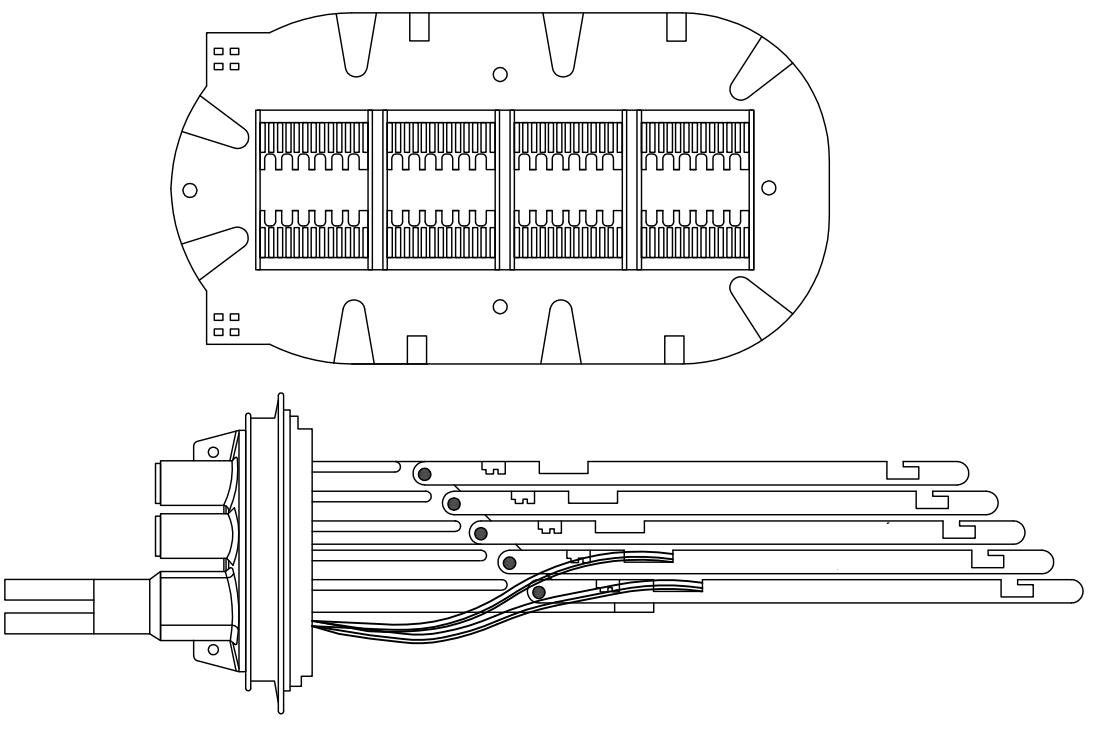
\includegraphics[width=0.5\linewidth]{../images/caixa_emenda_detalhe_bandejas.png}
  \end{figure}
\end{frame}

\begin{frame}{\ref{sec:estado_da_arte} - Estado da Arte | Redes Ópticas}
  \begin{figure}
    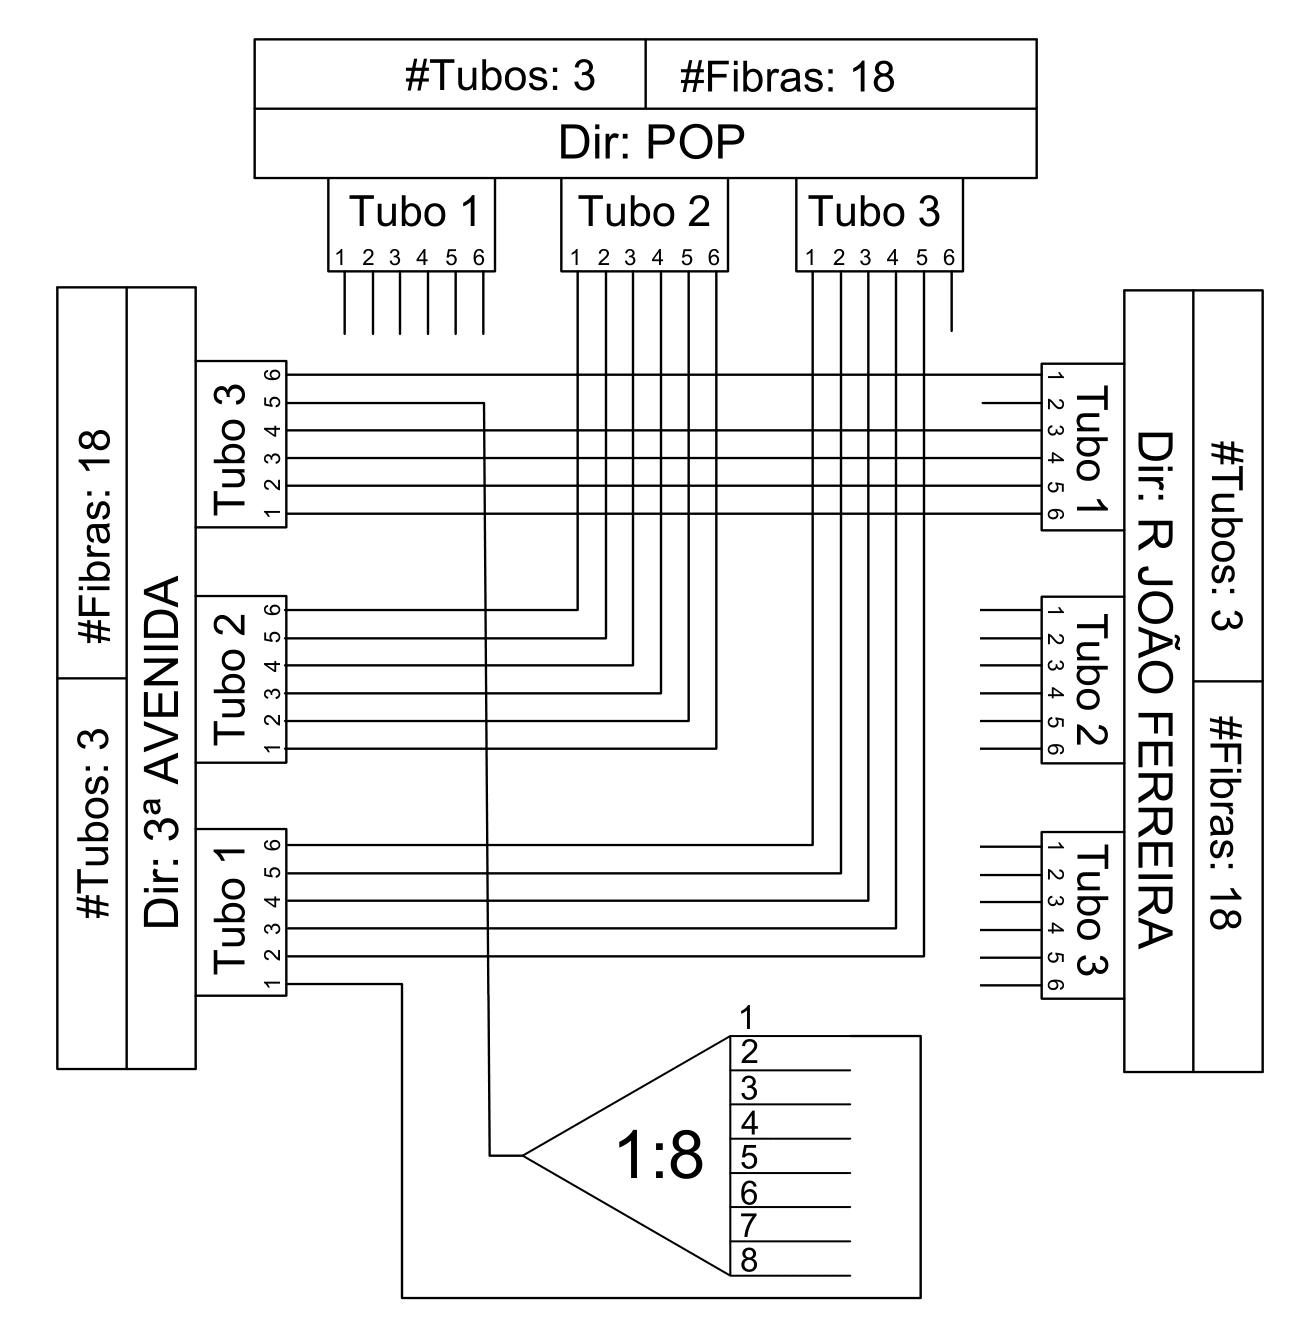
\includegraphics[width=0.45\linewidth]{../images/diagrama_fusoes.png}
  \end{figure}
\end{frame}

\begin{frame}{\ref{sec:estado_da_arte} - Estado da Arte | Algoritmos}
  \begin{itemize}
    \item São considerados dois algoritmos clássicos: Dijkstra e Bellman-Ford.
    \item O Algoritmo de Dijkstra encontra o caminho de menor custo em grafos com pesos não negativos.
    \item Bellman-Ford permite arestas com pesos negativos, mas apresenta maior complexidade temporal.
  \end{itemize}
\end{frame}

\begin{frame}{\ref{sec:estado_da_arte} - Estado da Arte | Algoritmo de Dijkstra}
  \begin{itemize}
    \item No contexto de redes óptica, Dijkstra é aplicável, pois o custo corresponde à distância, não havendo pesos negativos.
    \item A complexidade de tempo do Dijkstra envolve três operações principais: inserção, remoção e atualização de vértices na fila de prioridades.
    \item Com estrutura de fila baseada em lista, o algoritmo apresenta complexidade total $O(V^2 + EV)$.
  \end{itemize}

    \begin{alertblock}{Ponto de Atenção}
      O Algoritmo de Dijkstra não é ideal para longas sequências de nós, devido à necessidade de percorrer todo o ramo.
    \end{alertblock}
\end{frame}

\section{Escopo do Problema}\label{sec:escopo}
\begin{frame}{\ref{sec:escopo} - Escopo do Problema}
  \begin{enumerate}
    \item Elementos ativos são desconsiderados (i.e. DWDMs, OLTs).
    \item Multiplexação e conversores de onda são desconsiderados.
    \item Atenuação é desconsiderado.
    \item Considera-se uma fibra ocupada quando há um comprimento de onda associado a ela, ou seja, um $\lambda$ por alocação.
  \end{enumerate}
\end{frame}

\begin{frame}{\ref{sec:escopo} - Escopo do Problema | Pontos de Observação}
  \begin{itemize}
    \item Em redes novas, as fibras são geralmente alocadas de forma espelhada (do menor ao maior índice).
    \item Em falhas ou substituições temporárias de cabos, o "espelhamento" pode se perder, mas o retorno dos comprimentos de onda as mesmas fibras simplifica a reorganização.
  \end{itemize}
  \begin{figure}
    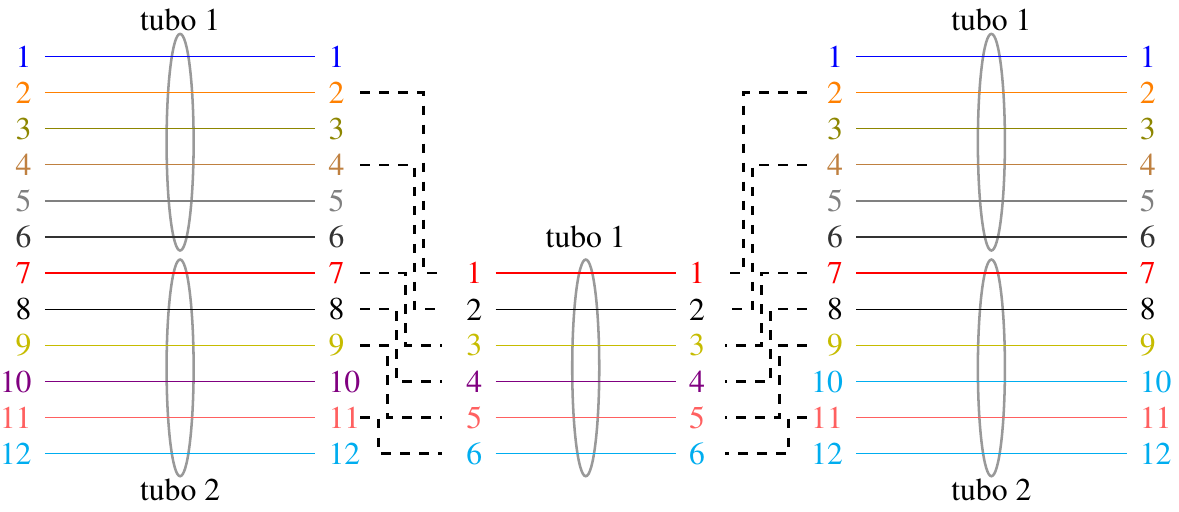
\includegraphics[width=0.70\linewidth]{../images/fluxo_reduzido.png}
  \end{figure}
\end{frame}

\begin{frame}{\ref{sec:escopo} - Escopo do Problema | Pontos de Observação}
  \begin{itemize}
    \item A alocação de fibras é um problema NP-completo, com crescimento combinatorial fatorial $O(n!)$ semelhante ao problema do caixeiro-viajante.
  \end{itemize}
  \begin{figure}
    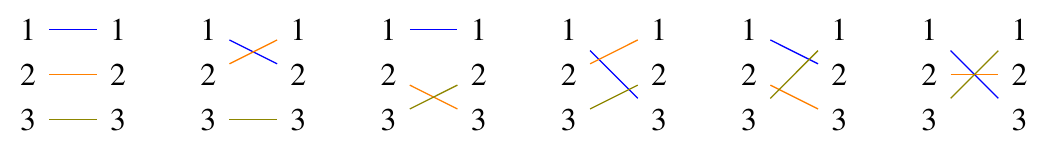
\includegraphics[width=0.80\linewidth]{../images/combinacoes_possiveis.png}
  \end{figure}
\end{frame}

\section{Estudo de Caso}\label{sec:estudo_de_caso}
\begin{frame}{\ref{sec:estudo_de_caso} - Estudo de Caso}
  \begin{itemize}
    \item Cálculo das $n$ melhores rotas: custo depende da implementação de Dijkstra / K-shortest.
    \item Análise de cada rota: espaço proporcional ao comprimento da maior rota (pilha de conexões) $\Rightarrow O(n)$ em termos práticos.
    \item A escolha de fibra é linear na quantidade de enlaces da rota (verificação por enlace).
  \end{itemize}
  \note{(40s) Comentar que heurística evita combinatorial blow-up da formulação exata, por isso é prática para redes de grande porte.}
\end{frame}

\begin{frame}{\ref{sec:estudo_de_caso} - Estudo de Caso | Resultados Esperados}
  \begin{itemize}
    \item Identificar rotas viáveis com melhor aproveitamento de fibras.
    \item Redução de bloqueios e manutenção do espelhamento físico nas bandejas.
    \item Simplicidade de integração com NMS e implementação em ferramentas como NetworkX/Cisco CML.
  \end{itemize}
  \note{(40s) Explicar cenários de uso: provisionamento automatizado, planejamento de rota em restauração, testes em ambiente simulado.}
\end{frame}

\begin{frame}{\ref{sec:estudo_de_caso} - Estudo de Caso | Limitações}
  \begin{itemize}
    \item Sem testes empíricos no artigo (falta validação em simulação/produção).
    \item Não trata múltiplos comprimentos de onda por fibra nem atenuação.
    \item Estratégia heurística pode não ser ótima em cenários altamente carregados.
  \end{itemize}
  \note{(30s) Ser crítico: indicar quando a heurística pode falhar e necessidade de comparação com outras abordagens.}
\end{frame}

\section{Conclusão}\label{sec:conclusao}
\begin{frame}{\ref{sec:estudo_de_caso} - Conclusão}
  \begin{itemize}
    \item Heurística integra cálculo de menor caminho com regras práticas de alocação de fibra.
    \item Boa relação entre simplicidade operacional e aplicabilidade prática.
    \item Serve como base para implementações e experimentos futuros.
  \end{itemize}
  \note{(30s) Reforçar contribuição conceitual e utilidade prática como ponto de partida.}
\end{frame}

\begin{frame}{Trabalhos Futuros}
  \begin{itemize}
    \item Implementação e avaliação em simulador (CML, NetworkX, OMNeT++).
    \item Extensão para múltiplos $\lambda$ por fibra (RWA completo) e inclusão de atenuação/distância.
    \item Comparação com heurísticas/algoritmos meta-heurísticos (GA, GRASP, etc.).
    \item Integração com dados reais de inventário e políticas de operação.
  \end{itemize}
  \note{(40s) Sugerir métricas para avaliação: taxa de bloqueio, utilização de fibra, tempo de alocação, custo de manutenção.}
\end{frame}

% \begin{frame}{Blocks of Highlighted Text}
%     In this slide, some important text will be \alert{highlighted} because it's important. Please, don't abuse it.
%
%     \begin{block}{Block}
%         Sample text
%     \end{block}
%
%
%     \begin{examples}
%         Sample text in green box. The title of the block is ``Examples".
%     \end{examples}
% \end{frame}

% \begin{frame}{Multiple Columns}
%     \begin{columns}[c] % The "c" option specifies centered vertical alignment while the "t" option is used for top vertical alignment
%
%         \column{.45\textwidth} % Left column and width
%         \textbf{Heading}
%         \begin{enumerate}
%             \item Statement
%             \item Explanation
%             \item Example
%         \end{enumerate}
%
%         \column{.45\textwidth} % Right column and width
%         Lorem ipsum dolor sit amet, consectetur adipiscing elit. Integer lectus
%         nisl, ultricies in feugiat rutrum, porttitor sit amet augue. Aliquam ut
%         tortor mauris. Sed volutpat ante purus, quis accumsan dolor.
%
%     \end{columns}
% \end{frame}
%
% \begin{frame}{Table}
%     \begin{table}
%         \begin{tabular}{l l l}
%             \toprule
%             \textbf{Treatments} & \textbf{Response 1} & \textbf{Response 2} \\
%             \midrule
%             Treatment 1         & 0.0003262           & 0.562               \\
%             Treatment 2         & 0.0015681           & 0.910               \\
%             Treatment 3         & 0.0009271           & 0.296               \\
%             \bottomrule
%         \end{tabular}
%         \caption{Table caption}
%     \end{table}
% \end{frame}
%
% \begin{frame}{Theorem}
%     \begin{theorem}[Mass--energy equivalence]
%         $E = mc^2$
%     \end{theorem}
% \end{frame}

\begin{frame}{Figure}
    Uncomment the code on this slide to include your own image from the same directory as the template .TeX file.
    %\begin{figure}
    %\includegraphics[width=0.8\linewidth]{test}
    %\end{figure}
\end{frame}

\nocite{*}

\setbeamertemplate{bibliography item}[triangle]
\begin{frame}[shrink=16]{Referências}
    \footnotesize
    \bibliographystyle{siam}
    \bibliography{../util/references.bib}
\end{frame}

\end{document}
